%
% Complete documentation on the extended LaTeX markup used for Insight
% documentation is available in ``Documenting Insight'', which is part
% of the standard documentation for Insight.  It may be found online
% at:
%
%     http://www.itk.org/

\documentclass{InsightArticle}

\usepackage[dvips]{graphicx}
\usepackage{cite}
\usepackage{url}

%%%%%%%%%%%%%%%%%%%%%%%%%%%%%%%%%%%%%%%%%%%%%%%%%%%%%%%%%%%%%%%%%%
%
%  hyperref should be the last package to be loaded.
%
%%%%%%%%%%%%%%%%%%%%%%%%%%%%%%%%%%%%%%%%%%%%%%%%%%%%%%%%%%%%%%%%%%
\usepackage[dvips,
bookmarks,
bookmarksopen,
backref,
colorlinks,linkcolor={blue},citecolor={blue},urlcolor={blue},
]{hyperref}
\graphicspath{{fig/}}

\usepackage{subfigure}
\usepackage{amsthm}

\theoremstyle{plain}
\newtheorem*{note}{Note}

\def \ie {\textit{i.e. }}
\def \etc {\textit{etc. }}
%  This is a template for Papers to the Insight Journal.
%  It is comparable to a technical report format.

% The title should be descriptive enough for people to be able to find
% the relevant document.
\title{Surface Meshes Incremental\\
Decimation Framework}

% Increment the release number whenever significant changes are made.
% The author and/or editor can define 'significant' however they like.
\release{0.01}

% At minimum, give your name and an email address.  You can include a
% snail-mail address if you like.
\author{Arnaud Gelas, Alexandre Gouaillard\\
and Sean Megason}
\authoraddress{Department of System Biology, Harvard Medical School,\\
Boston, MA 02115, USA}
% \email{}

\begin{document}


\ifpdf
\else
   %
   % Commands for including Graphics when using latex
   %
   \DeclareGraphicsExtensions{.eps,.jpg,.gif,.tiff,.bmp,.png}
   \DeclareGraphicsRule{.jpg}{eps}{.jpg.bb}{`convert #1 eps:-}
   \DeclareGraphicsRule{.gif}{eps}{.gif.bb}{`convert #1 eps:-}
   \DeclareGraphicsRule{.tiff}{eps}{.tiff.bb}{`convert #1 eps:-}
   \DeclareGraphicsRule{.bmp}{eps}{.bmp.bb}{`convert #1 eps:-}
   \DeclareGraphicsRule{.png}{eps}{.png.bb}{`convert #1 eps:-}
\fi


\maketitle


\ifhtml
\chapter*{Front Matter\label{front}}
\fi


% The abstract should be a paragraph or two long, and describe the
% scope of the document.
\begin{abstract}
\noindent
When dealing with meshes, it is often preferable to work with a lower resolution mesh for computational time purpose, display. The process of reducing a given mesh, \emph{mesh decimation}, is thus an important step in most of pipeline dealing with meshes. \emph{Incremental decimation algorithms}, the most popular ones, consists of iteratively removing one point of the mesh, by Euler operations such as vertex removal or edge collapse. Here we focus on edge collapse based decimation approaches and propose a general framework based on a surface mesh data structure (\code{itk::QuadEdgeMesh}~\cite{itkQE}). Our implementation intends to be as general and as flexible as possible. Indeed it can theoretically be applied on any polygonal mesh\footnote{The measure needs to be defined in accordance.}; the measure, functional to be optimized at each iteration, the objective to be reached, and optional methods like point relocation to enhance the geometry of the resulting mesh, are given by the user. We provide here two specific implementations: \code{itk::QuadEdgeMeshSquaredEdgeLengthDecimation} and \code{itk::QuadEdgeMeshQuadricDecimation}, that could be used as example to implement additional algorithms.
\end{abstract}

\tableofcontents

\section{Introduction}
With current developments of acquisition techniques, generated surface meshes can be really large (from few hundred thousand to few hundred million polygons). When dealing with these meshes, users usually prefer working with a lower resolution mesh than the original one, and algorithms to reduce the number of simplices (points, edges, faces) in a given mesh are generally referred as \emph{mesh decimation algorithms}. There is no global solution, and depending on the user needs the decimation process may be completely different. For example one may want to focus on preserving the geometrical approximation, or some given characteristics such as normals, curvatures, or attributes...

Decimation algorithms can be classified into three different approaches: \textit{(i)} \emph{clustering}, \textit{(ii)} \emph{resampling} or \emph{remeshing}, and \textit{(iii)} \emph{incremental decimation}. Among these three kind of approaches, incremental decimation methods are certainly the most popular ones since it generally provides output meshes with higher quality.

\section{Design}
Based a $n$D 2-manifold mesh data structure available in itk (\code{itk::QuadEdgeMesh}~\cite{itkQE}), our design intends to be as flexible and general as possible for edge-collapse based decimation (see Figure~\ref{fig:merge_relocation}). To this end, depending on the application and the user needs, several informations are required to develop his own decimation method:
\begin{itemize}
 \item the cost function which returns the cost of a given edge.
 \item the way the cost function should be optimized\footnote{Note that the optimization is performed with a greedy algorithm.}: \textit{minimization or maximization?}
 \item the possible relocation of resulting point after edge collapse operation. \textit{Is there any relocation procedure? How to determine this new location?}
 \item if mesh normal inversions are allowed,
 \item if topological changes are allowed,
 \item the criterion to stop the decimation process.
\end{itemize}

\subsection{Edge Cost Function}
The cost function, error, or metric computation for a given edge \code{OutputQEType* iEdge} is a pure virtual method of
\code{itk::QuadEdgeMeshEdgeMergeDecimationFilter}, and must be implemented in inherited classes.

\begin{verbatim}
  virtual MeasureType MeasureEdge( OutputQEType* iEdge ) = 0;
\end{verbatim}


\subsection{Optimization}
As mention previously, we assume that the cost function can be minimized or maximized by a greedy algorithm. After one edge is collapsed, the cost of its neighbors may be affected by such operation (see Figure~\ref{fig:merge_relocation}). Therefore the container should allow user to modify the cost of internal elements. This is done by using a mutable priority queue container \code{itk::PriorityQueueContainer}~\cite{itkPriorityQueueContainer}. The element (\ie edge) with the highest priority (\ie cost), or lowest priority, is popped from the container and collapsed; then priority of elements affected by this operation are updated.

The optimization procedure is given by the type of mutable priority queue used, and is thus given as template argument.

\subsection{Point Relocation}

\begin{figure}[tb]
  \centering
  \subfigure[]{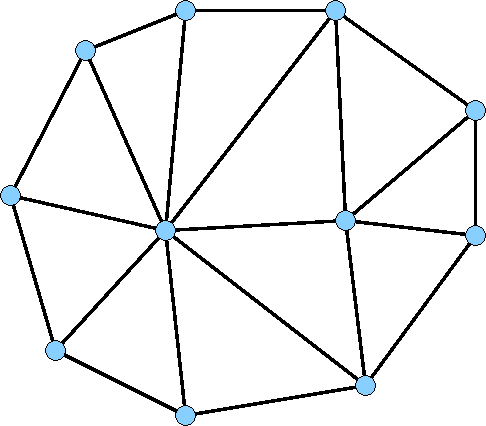
\includegraphics[width=0.3\textwidth]{merge0.png}}
  \subfigure[]{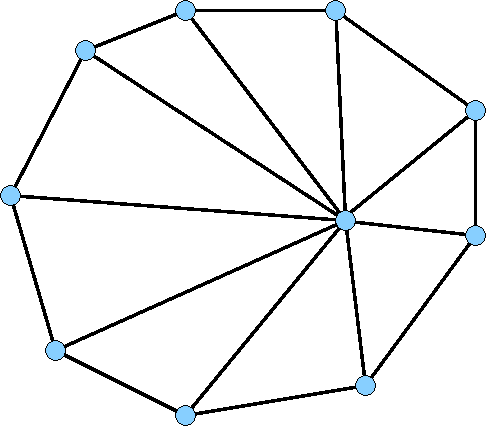
\includegraphics[width=0.3\textwidth]{merge1.png}}
  \subfigure[]{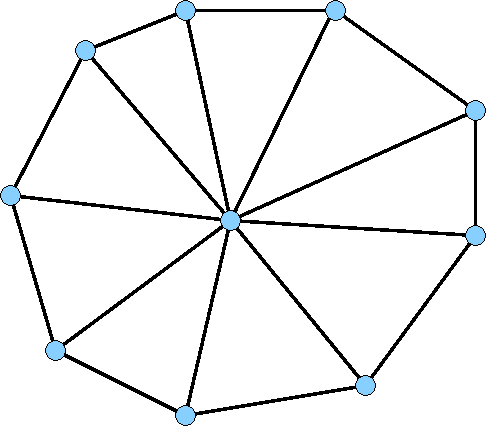
\includegraphics[width=0.3\textwidth]{merge2.png}}
  \caption{From the initial configuration~(a), the central edge is contracted~(b) and the remaining vertices can be relocated~(c).}
  \label{fig:merge_relocation}
\end{figure}

In some cases, after merging two vertices user may want to move the remaining vertex to a new position which minimizes the cost function of neighbor edges, or relaxes the edge collapse procedure (see Figure~\ref{fig:merge_relocation}). This method is declared in \code{itk::QuadEdgeMeshEdgeMergeDecimationFilter} as pure virtual method, and must be implemented in inherited classes.

\begin{verbatim}
  virtual OutputPointType Relocate( OutputQEType* iEdge ) = 0;
\end{verbatim}


\subsection{Mesh Inversion Prevention}
Edge contraction do not necessarily preserve the orientation of faces in a vicinity of the one considered. For instance, it is possible to merge two points and cause some neighboring faces to fold over on each other. Thus, user may want to avoid such configuration during the edge merging~\cite{Ronfard96}.

To our knowledge, this feature is not available in VTK decimation implementations. However user should be aware that preventing mesh inversion can be performed but at a cost that can slow down the decimation procedure.

\subsection{Topological Modifications}
Some rules can be applied to edge contraction to allow or avoid merge of boundaries, change of genus, \ie anything which could alter the Euler characteristic.

\begin{note}
 The implementation will be provided in a next release of this framework.
\end{note}


\subsection{Stopping Criterion}
Depending on user needs, or on the application, several stopping criteria can be considered. For example, one can fix the final number of faces, points, or an objective value to be reached by the cost function. At each iteration, the algorithm checks if the stopping condition is fulfilled or not. To provide more flexibility, the stopping criterion is given as template argument. One can make his own criterion to stop the algorithm by inheriting from \code{itk::QuadEdgeMeshDecimationCriterion}, and providing the implementation of the pure virtual method.

\begin{verbatim}
template<
  class TMesh,                          // Mesh Type to be processed
  typename TElement  = unsigned long,   // Type of the last processed element
  typename TMeasure = double,           // Type of the cost
  class TPriorityQueueWrapper =
    MinPriorityQueueElementWrapper< typename TMesh::QEType*,
                                    std::pair< bool, TMeasure > >
  // Type for the PriorityQueueContainer wrapper
  // Note: this last line provides the information if it is a min or max
  //priority queue
  >
class QuadEdgeMeshDecimationCriterion
{
public:
  ...

  virtual bool is_satisfied( MeshType* iMesh,
                             const ElementType& iElement,
                             const MeasureType& iValue) const=0;
};
\end{verbatim}

Here, we provide some basic criteria that could directly be used:
\begin{itemize}
 \item \code{itk::NumberOfPointsCriterion} where a number of points is given,
 \item \code{itk::NumberOfFacesCriterion} where a number of faces is given,
 \item \code{itk::MeasureBoundCriterion} where a bound on the cost function is given.
\end{itemize}

\subsection{Note on edge collapse and delete point}
The edge collapse method have already been implemented through the method \code{Evaluate} of the class \code{itk::QuadEdgeMeshEulerOperatorJoinVertexFunction}. Interested readers should note that after merging two points, the unused point is removed from the points container leading to non-contiguous point identifiers in the container. As long as the code is only using \code{itk::QuadEdgeMesh} it does not matter, but as soon as the mesh must be saved in a mesh format with contiguous assumptions on the identifier some problems can occur. Indeed when removing one point from the container and saving or displaying the mesh with \code{VTK} some problem occurs: edges and triangles that are not supposed to exist are displayed. This issue is solved by calling \code{itk::QuadEdgeMesh::SqueezePointIds}. Note that this is done in the decimation framework at the end of the \code{GenerateData} method.

\section{Examples of implementation}
In this section, we present two algorithms for mesh decimation. The first one removes iteratively the shortest edge of the mesh and can be applied for any polygonal mesh. The second one is a quadric based decimation~\cite{Garland97:QEM}, which provide a much better approximation of the original mesh, can only be applied on triangular meshes.
\subsection{Squared Edge Length}
The most basic implementation, we provide remove the shortest edge at each iteration until the given criterion is fulfilled. Therefore, we only needed to implement:
\begin{itemize}
 \item \code{MeasureEdge} which returns the squared edge length of a given edge.
 \item \code{Relocate} which relocate the point in the middle of the given edge if user wants to relocate the remaining point.
\end{itemize}

\subsection{Quadrics}
A more interesting example is the quadric based decimation~\cite{Garland97:QEM} (see Figure~\ref{fig:bunny_quadric}), where the element with the lowest quadric energy term is collapsed at each iteration, until the given criterion is fulfilled. Therefore, we only needed to implement:
\begin{itemize}
 \item \code{MeasureEdge} which returns the quadric energy term for a given edge.
 \item \code{Relocate} which relocate the point where the quadric energy term is minimal.
\end{itemize}

\section{Customization}
Make your own edge-collapsed decimation is quite simple, only few methods (at least two) need to be implemented in a class which inherits from \code{itk::QuadEdgeMeshEdgeMergeDecimationFilter}, and depending on the aim to be achieved a specific criterion class must be implemented (or one we provide can be used as well).

\section{Usage}
Here we show how to use the implementation of our framework we provide. First we need to define some general type and read a mesh:

\begin{verbatim}
  typedef double Coord;
  const unsigned int Dimension = 3;

  // Declaration of the type of Mesh
  typedef itk::QuadEdgeMesh< Coord, Dimension > MeshType;

  // Here read a mesh from a file
  ...
\end{verbatim}

\subsection{Squared Edge Length}

\begin{verbatim}
  // Declaration of the stopping criterion
  // By default the cost function is to be minimized
  typedef itk::NumberOfFacesCriterion< MeshType > CriterionType;

  // Here we assume that the user wants a mesh with N faces in output.
  // N is given by user
  CriterionType::Pointer criterion = CriterionType::New();
  criterion->SetTopologicalChange( false );
  criterion->SetNumberOfElements( N );

  // Declaration of the Decimation filter
  // MeshType as input and output, and criterion
  typedef itk::QuadEdgeMeshSquaredEdgeLengthDecimation< MeshType, MeshType,
    CriterionType > DecimationType;

  DecimationType::Pointer decimate = DecimationType::New();
  decimate->SetInput( mesh );
  decimate->SetCriterion( criterion );
  // Here we allow the relocation procedure
  decimate->SetRelocate( true );
  decimate->Update();

  MeshType::Pointer mesh = decimate->GetOutput();
\end{verbatim}

\subsection{Quadrics}

\begin{figure}[tb]
  \centering
  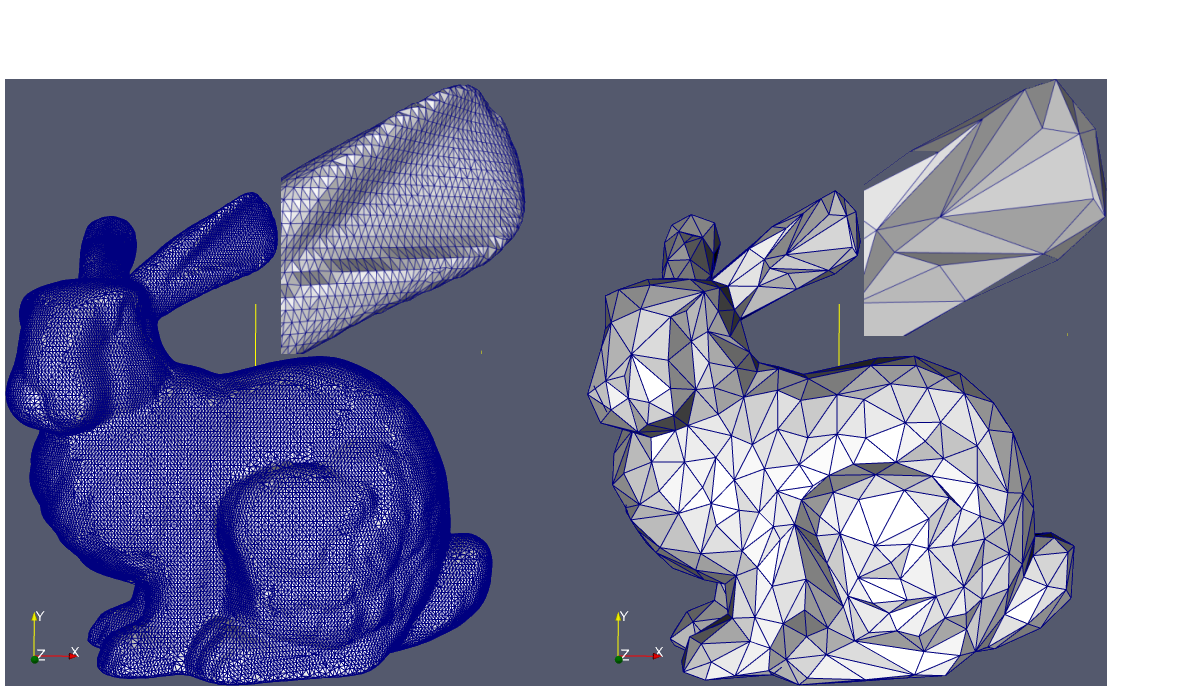
\includegraphics[width=1.\textwidth]{bunny_comp}
  \caption{Stanford bunny mesh on the left (69k faces), and the resulting mesh after quadric decimation (1k faces).}
  \label{fig:bunny_quadric}
\end{figure}

\begin{verbatim}
  // Declaration of the stopping criterion
  // By default the cost function is to be minimized
  typedef itk::NumberOfFacesCriterion< MeshType > CriterionType;

  // Here we assume that the user wants a mesh with N faces in output.
  // N is given by user
  CriterionType::Pointer criterion = CriterionType::New();
  criterion->SetTopologicalChange( true );
  criterion->SetNumberOfElements( N );

  // Declaration of the Decimation filter
  typedef itk::QuadEdgeMeshQuadricDecimation< MeshType, MeshType,
    CriterionType > DecimationType;

  DecimationType::Pointer decimate = DecimationType::New();
  decimate->SetInput( mesh );
  decimate->SetCriterion( criterion );
  decimate->Update();

  MeshType::Pointer mesh = decimate->GetOutput();
\end{verbatim}

\section{Software Requirements}

You need to have the following software installed:

\begin{itemize}
  \item Insight Toolkit $\geq$ 3.7.0 (Revision $\geq$ 1.2737) compiled with USE\_REVIEW ON.
  \item CMake $\geq$ 2.4
\end{itemize}

\section*{Acknowledgment}
The Stanford bunny model is from Stanford University Computer Graphics Laboratory.\\

This work was funded by a grant from the NHGRI (P50HG004071-02) to found the Center for in toto genomic analysis of vertebrate development.

%%%%%%%%%%%%%%%%%%%%%%%%%%%%%%%%%%%%%%%%%
%
%  Insert the bibliography using BibTeX
%
%%%%%%%%%%%%%%%%%%%%%%%%%%%%%%%%%%%%%%%%%

\bibliographystyle{plain}
\bibliography{decimation}

\end{document}

